\documentclass[../slides]{subfiles}

\begin{document}
    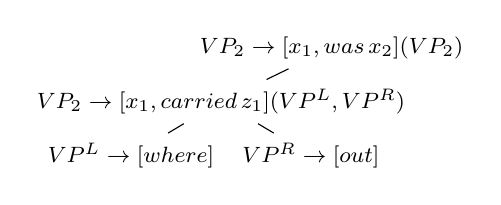
\begin{tikzpicture}[
            level distance=4.5ex,
            every node/.style={font=\footnotesize}
        ]
        \node (vp1) {\(VP_2 \to [x_1, \text{was}\, x_2] (VP_2)\)}
        [sibling distance=6.5em]
        child { node[xshift=-4em] (vp2) {\(VP_2 \to [x_1, \text{carried}\, z_1] (VP^L, VP^R)\)}
            child { node (term0) {\(VP^L \to [\text{where}]\)}}
            child { node (term5) {\(VP^R \to [\text{out}]\)}}};
    \end{tikzpicture}
\end{document}